\chapter{Validación de un pipeline para la identificación de variantes}

Los pipelines son un componente integral de la secuenciación de siguiente generación (NGS), para el procesamiento de los datos en bruto y detectar las alteraciones genómicas que tienen un impacto en la salud de un paciente, por lo tanto se hace necesario el desarrollo, validación y monitoreo de los pipelines  para disminuir los errores de la identificación de variantes \cite{Roy2018}. \\

En este capítulo se presenta el proceso para validar un pipeline que permitió la  identificación de variantes a partir de datos de secuenciación de siguientes generación (NGS), donde se utiliza datos públicos para validar la calidad  de las variantes. El capítulo se encuentra organizado en identificación de variantes, datos, estrategias del pipeline, resultados y validación, discusión y conclusiones. 

\section{Identificación de variantes}

Los pipelines bioinformaticos para NGS son comúnmente desarrollados en una plataforma específica y pueden ser adaptados según las necesidades del laboratorio, la mayoría de los pipelines consisten en los siguientes pasos \cite{Roy2018}:

\begin{enumerate}[1.]
	\item Generación de secuencias. 
	\item Alineamiento de las secuencias. 
	\item Llamado de variantes. 
	\item Filtrado de variantes. 
	\item Anotación de variantes. 
	\item Priorización de variantes. 
\end{enumerate}
 
La eficiencia de la identificación de variantes depende de la exactitud del llamado de las bases (la identificación correcta de cada nucleótido dentro de la secuencia), esto se realizó debido a que durante el proceso de secuenciación  se identifican los nucleótidos de manera incorrecta, se considera que al momento la exactitud de ese llamado esta alrededor del 99. 5\% \cite{Tetreault2015}. Teniendo en cuenta lo anterior es recomendable  priorizar la sensibilidad (Buscar tantas variantes como sea posible para evitar perder cualquier variante) sobre la especificidad (Limita la proporción de falsos positivos en un conjunto de variantes) \cite{Auwera2014}.  \\

Para el presente trabajo se realizaron mediciones de la calidad de las secuencias y el mapeo, post-alineamiento y el llamado de variantes, siguiendo las buenas prácticas para el llamado de variantes \cite{Fisch2015}. Teniendo en cuenta que existen múltiples herramientas para realizar el llamado de variantes, tanto de uso privado como open source, que permiten  seguir las buenas prácticas de identificación de variantes, se hace necesario integrar las diversas herramientas para poder obtener las datos de buena calidad. Y surge la pregunta de ¿cuáles de todos los métodos y las herramientas son la más apropiada para hacer el llamado de variantes en exones? \cite{Bao2014}\cite{Cornish2015}. \\

Para dar respuesta a esta pregunta se ha seguido la propuesta de buenas prácticas para el llamado de variantes propuesto por el Broad Institute que incluyen el procesamiento de los datos, el mapeo (Alinemaiento de las secuencias), descubrimiento de variantes y la recalibración del set de variantes obtenidas. Para poder llevar acabo la adecuada implementación se hace necesario la utilización de HPC (Computación de alto desempeño) donde la utilización de un clúster para bioinformática presentan una gran apoyo para el procesamiento y análisis de datos incluso es un requisito de algunos módulos para poder implementarse adecuadamente \cite{Fisch2015}. 

\section{Datos}

Los datos que fueron procesados en el presente trabajo son secuencias de 4813 exones humanos se obtuvieron de kit de Illumina TruSight One en muestras de sangre periférica. Estos datos  fueron donados por el Centro de Investigaciones en Genética Humana y Reproductiva GENETIX S. A. S dirigido por la Dra Claudia Serrano Médico Genetista. \\

Para la validación del pipilene se corrió un exoma público de  NA12878-NGv3-LAB1360 que pertenece a una mujer que tiene una variación en el gen CYP2C19 donde tiene una transición de una Guanina por una Adenina en la posición 681 del exón 5, que causa un cambio en el marco de lectura del ARNm a partir del aminoácido 215 y produce un códon de parada prematuro en 20 aminoácidos corriente abajo produciendo una proteína no funcional (\textit{Información obtenida de Coriell Institute for medical reseach}). \\

Se descargó el archivo bed para filtrar las variantes que se encuentran dentro del genoma completo de la muestra para obtener solo exones del NCBI para el genoma hg19. También se realizó una obtención de variantes a partir de un exoma completo público de la muestra NA12878, los datos fueron obtenidos via ftp en la siguiente direcciones:\\
\\
{\texttt{ https://s3. amazonaws. com/bcbio\_nextgen/NA12878-NGv3-LAB1360-A\_1. fastq. gz}\\
\\
{\texttt{ https://s3. amazonaws. com/bcbio\_nextgen/NA12878-NGv3-LAB1360-A\_2. fastq. gz}}\\
\\
Y el archivo bed para filtrar las variantes que se encuentran dentro del genoma completo de la muestra se obtuvo de la siguiente pagina para el genoma hg19: \\
\\
\texttt{ftp://ftp-trace. ncbi. nlm. nih. gov/giab/ftp/data/NA12878/analysis/}\\
\\
\texttt{Illumina\_PlatinumGenomes \_NA12877\_NA12878\_09162015/hg19/8. 0. 1/NA12878/} 

\section{Estrategias del pipeline}

Existen una serie de pasos para la obtención de variantes la obtención de la calidad de las secuencias y preprocesamiento como la remoción de adaptadores y de nucleótidos con baja calidad (que son erroneamente identificados por el secuenciador), posteriormente sigue el mapeo, post-alineamiento, llamado de variantes, anotación y priorización \cite{Bao2014}. \\

Se utilizó como base el módulo de omics-pipe propuesto por Fish y colaboradores \cite{Fisch2015}, que presenta el pipeline acorde con las buenas prácticas para el llamado de variantes. Para el presente trabajo se adicionó el filtrado específico de variantes según GATK y la parte de anotación de variantes con wAnnovar como se muestra  en la figura \ref{fig:pipeline2}. 

\begin{figure}[H] 
	\centering
	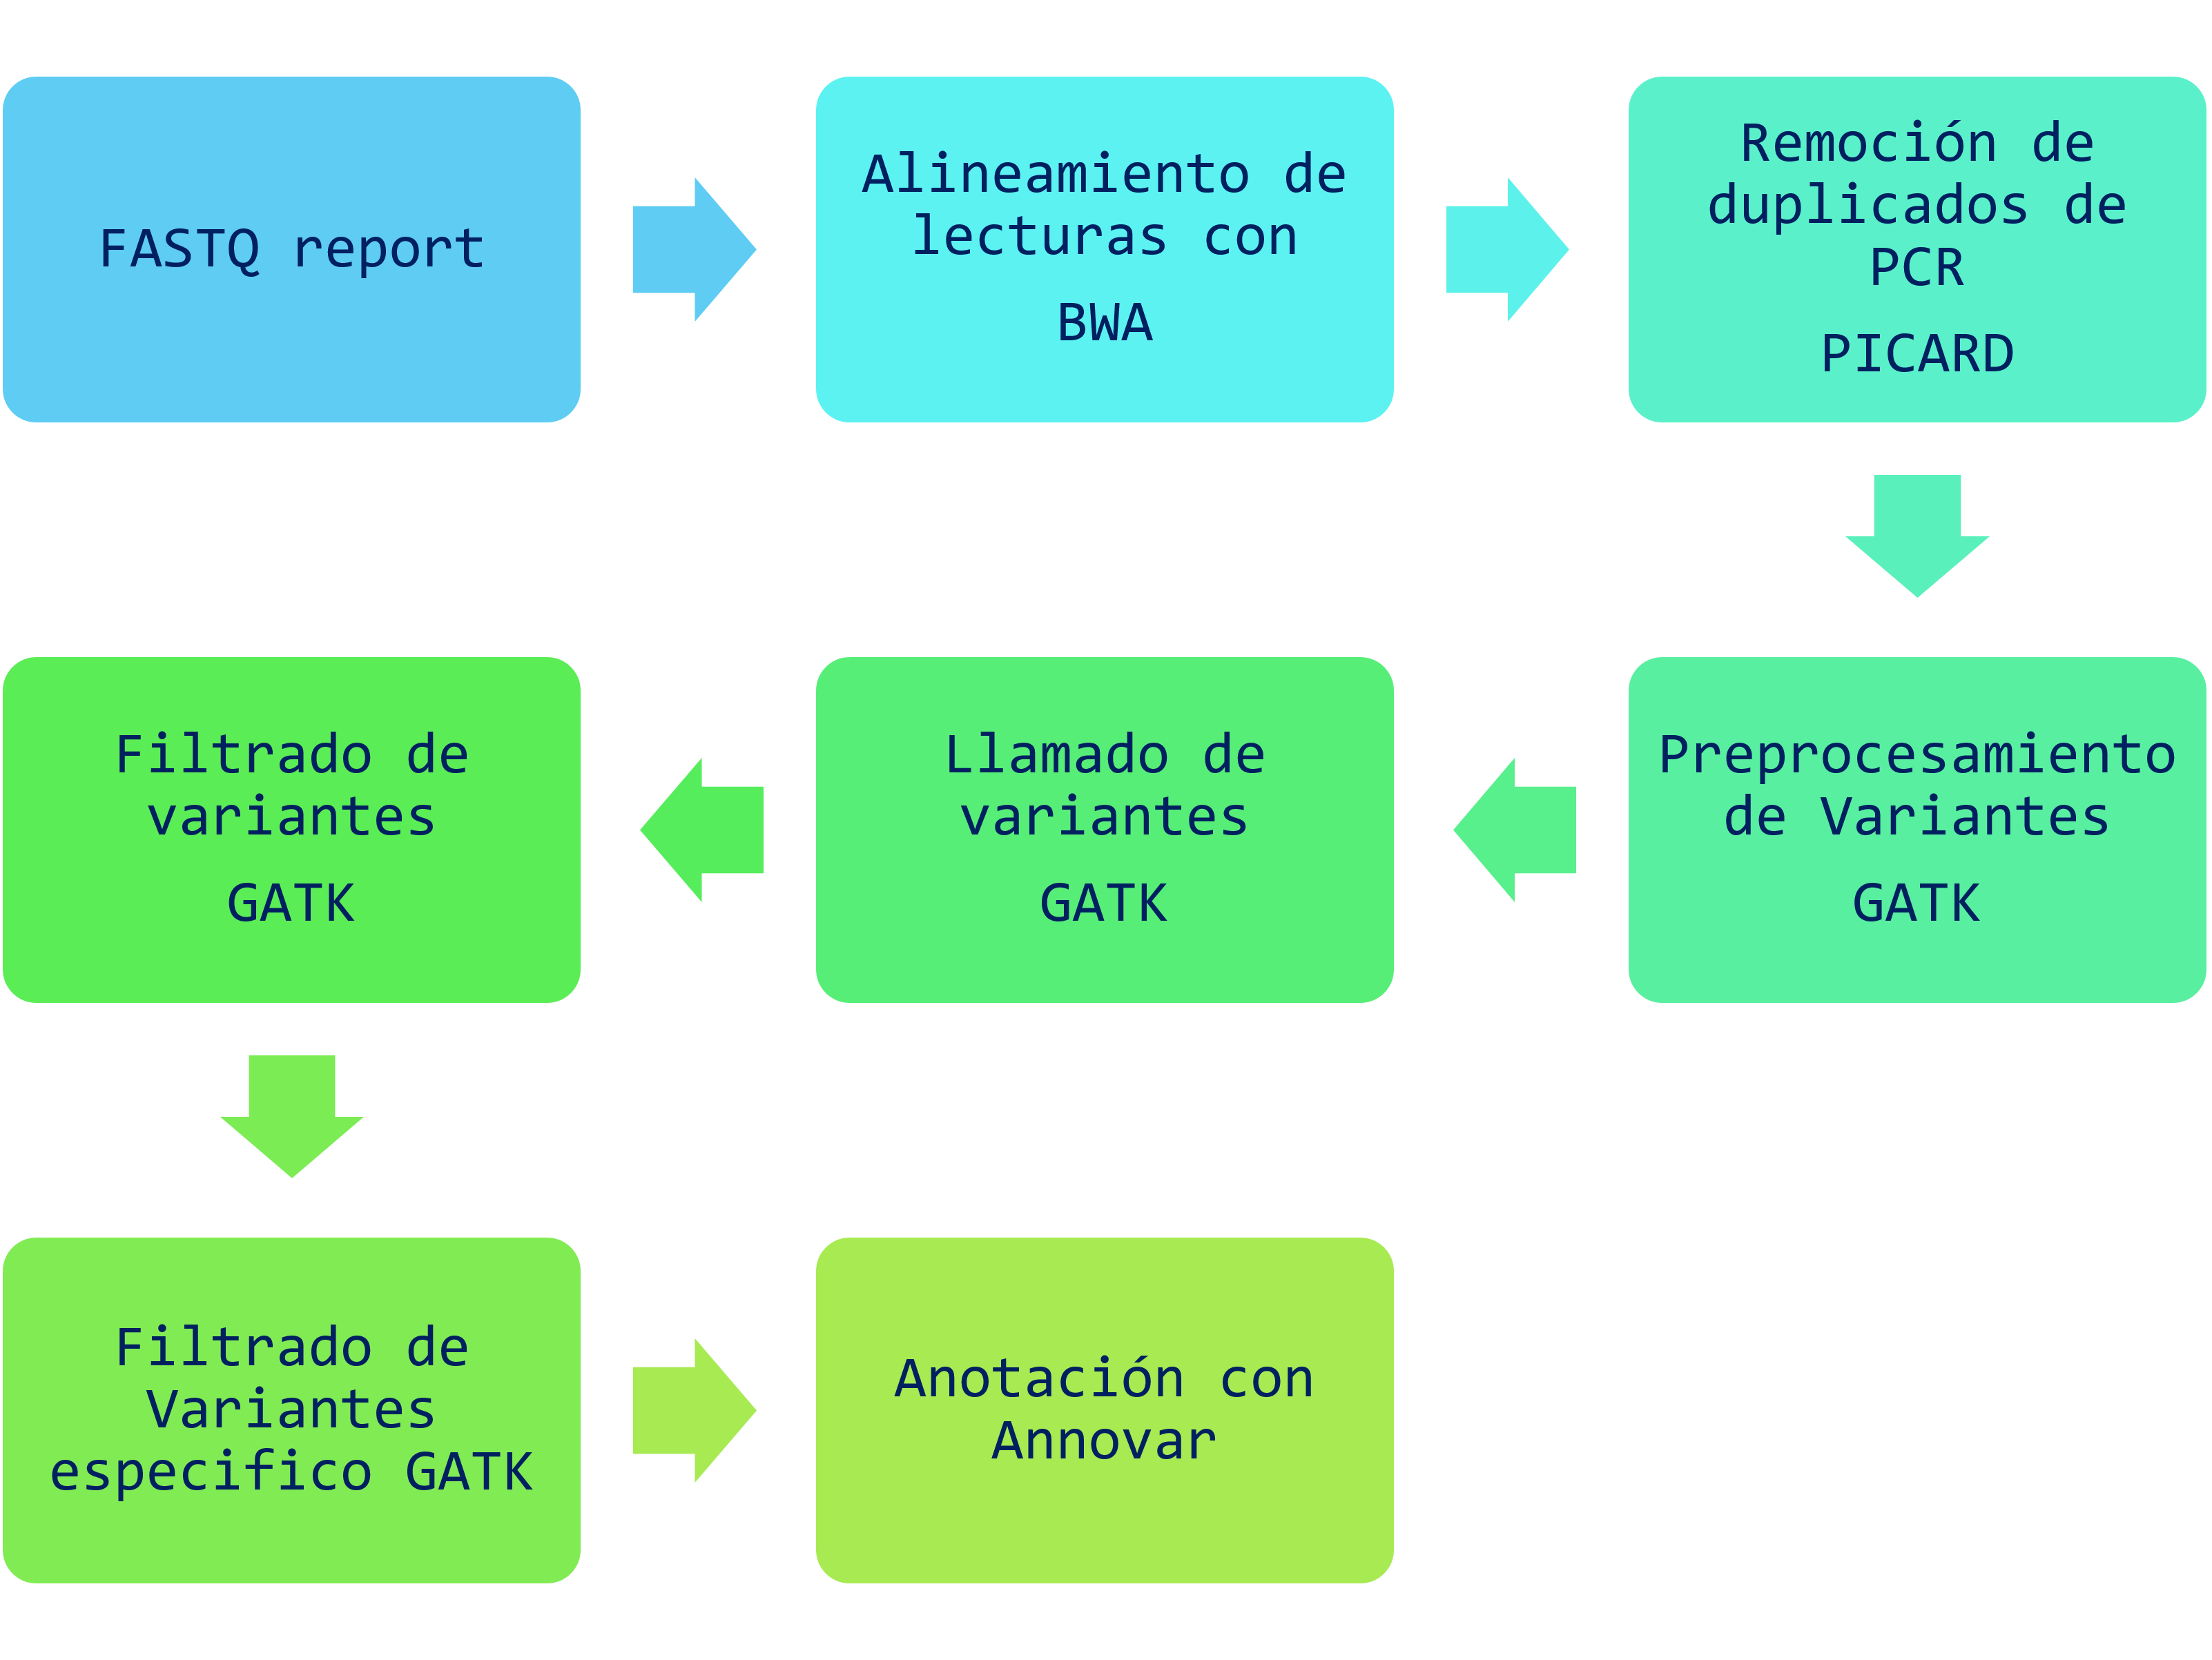
\includegraphics[width=0.6\textwidth]{Kap2/pipeline1}
	\caption{Pipeline base para el llamado de variantes. } \label{fig:pipeline2}
\end{figure}


\subsection*{Herramientas computacionales}
	
	Las herramientas bioinformáticas seleccionadas se implementaron en un clúster \footnote{El clúster utilizado fue prestado por la Universidad de los Andes} que cuenta con las siguientes características:
	
	\begin{itemize}
		\item[$\Rightarrow$] Un nodo master con 2 procesadores Intel Xeon E5-2695 – 24 cores 48 con HT / 192 GB RAM (230Gflops), 300 GB de Disco duro. 
		\item[$\Rightarrow$] Se tienen 19 nodos de trabajo con 2 procecesadores  Intel Xeon E5-2695 – 24 cores 48 con HT / 192 GB RAM (4. 378Tflops), 300 GB de de Disco duro. 
		\item[$\Rightarrow$] Se cuentan con otros 7 nodos de trabajo con 4 procesadores AMD Opteron 6282 SE – 64 cores / 128 GB RAM (3. 659Tflops), 200 GB de Disco duro. 
		
		\item[$\Rightarrow$] 1 GPU tesla K20 como nodo de trabajo con 2 Procesores  Intel Xeon X5690 - 12 cores / 192 GB RAM (3. 659Tflops), 1. 6 TB de Disco duro. 
		
	\end{itemize}
	
Se instaló el módulo para python de omics-pipe, para python 2 con la herramienta de R y las librerías que solicita omics-pipe\cite{Fisch2015}. El algoritmo BWA-MEN samtools, vcftools, GATK 3. 5, picard, FASTQC y pbs-drmma. Una vez instalados los programas se procesaron las muestras dentro del clúster.  


\section{Resultados y validación}
	\subsection*{Reporte FASTQC}}

Este reporte utilizando la herramienta FASTQC presenta inicialmente un resumen del estado de las secuencias obtenidas, ya que toma el archivo fastq y lee las métricas de calidad de cada una de las bases y genera un reporte general en formato HTML. Ya que es interactivo y genera varios módulos \cite{Babraham2016}. \\

Este reporte no presenta fallas dentro del análisis. A continuación se muestra un el primer módulo del reporte FASTQ obtenido de un dato experimental de una secuenciación de 4813 genes que resume el estado general de las lecturas obtenidas para este caso, la figura \ref{fig:fastq2} muestra que la calidad de las secuencias es mayor a 30, el reporte general también muestra que no hay secuencias adaptadoras, que presenta una distribución media del largo de las secuencias aceptable y que no hay secuencias sobre representadas.  \\

\begin{figure}[H]
	\centering
	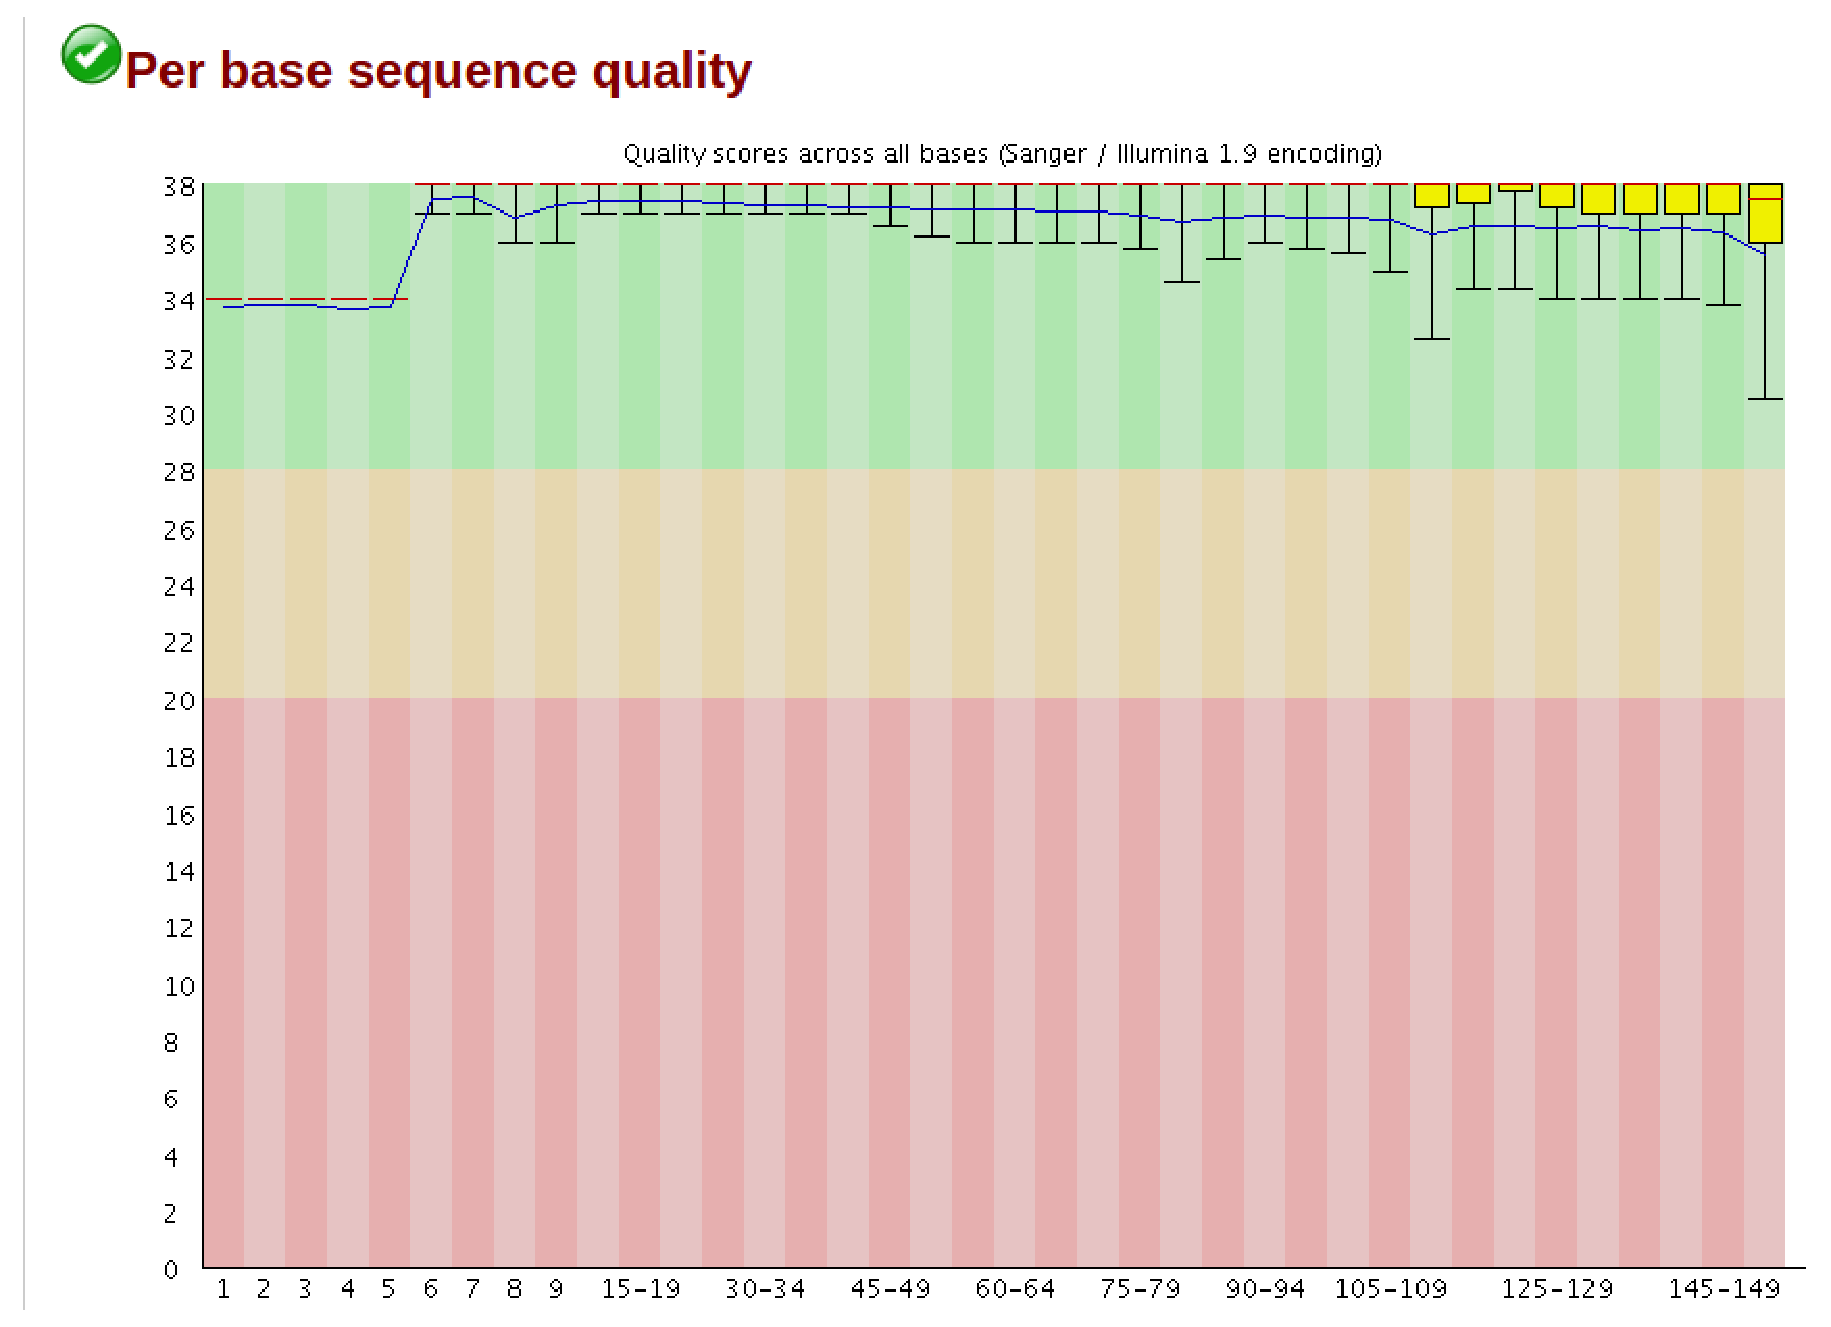
\includegraphics[width=0.4\textwidth]{Kap2/fastq2}
	\caption{Calidad del llamado de bases en una secuencia Estadísticas básicas del reporte FASTQ} \label{fig:fastq2}
\end{figure}

Para el caso de esta muestra la calidad es óptima en todos los datos obtenidos y no requieren de ningún tipo de ``trimming" ya que la mayoría de las posiciones dentro de la secuencia se encuentran por encima del un valor por encima de 34 y el cual el valor mínimo es 20 (este valor representa el ($Q_{PHARED}$) que implementa el secuenciador \cite{Babraham2016}. \\ 

\subsection*{Variantes de illumina vs variantes de Omics}

Inicialmente se obtuvieron 63515 variantes una vez que se ejecuto el pipeline de omics para la obtención de variantes, siguiendo los protocolos de buenas prácticas y los protocolos de GATK quienes recomiendan generar variantes altamente sensibles y poco precisas, esto con el fin de no perder variantes que se encuentren dentro de las secuencias obtenidas, por ello se muestra una gran cantidad de variantes que no corresponden con las variantes verdaderas \cite{Auwera2014}. Dentro del pipeline solo se encuentra el proceso de llamado de variantes y no el proceso de filtrado de las mismas y que debió ser implementado de manera manual. A partir de la aplicación del pipeline se obtuvieron resultados representado en el cuadro \ref{tabla:final}. 

\begin{table}[htb]
	\centering
	\begin{tabular}{|l|l|l|l|l|}
		\hline
		& \multicolumn{4}{c|}{\textbf{Variantes}} \\
		\cline{2-5} 
		& SNP  & Indels & Desconocida & Total \\ \cline{2-5}
		\hline 
		\multirow{1}{4cm}{Variantes Omics} & 54538 & 8855 & 122 & 63515 \\ \cline{2-5}
		\hline 
		\multirow{1}{4cm}{Variantes Calibradas} & 10425 & 828 & 44 & 11297 \\ \cline{2-5}
		\hline
		\multirow{1}{4cm}{Variantes Illumina} & 9601 & 436 & 28 & 10065 \\ \cline{2-5}
		\hline
	\end{tabular}
	\caption{Variantes obtenidas al aplicar pipeline.}
	\label{tabla:final}
\end{table}

De las variantes sin ``hard filtering" se obtuvieron 54538 SNP, Indels 8855 y 122 variantes desconocidas, que se presentan en la figura \ref{fig:omics}: 

\begin{figure}[H]
	\centering
	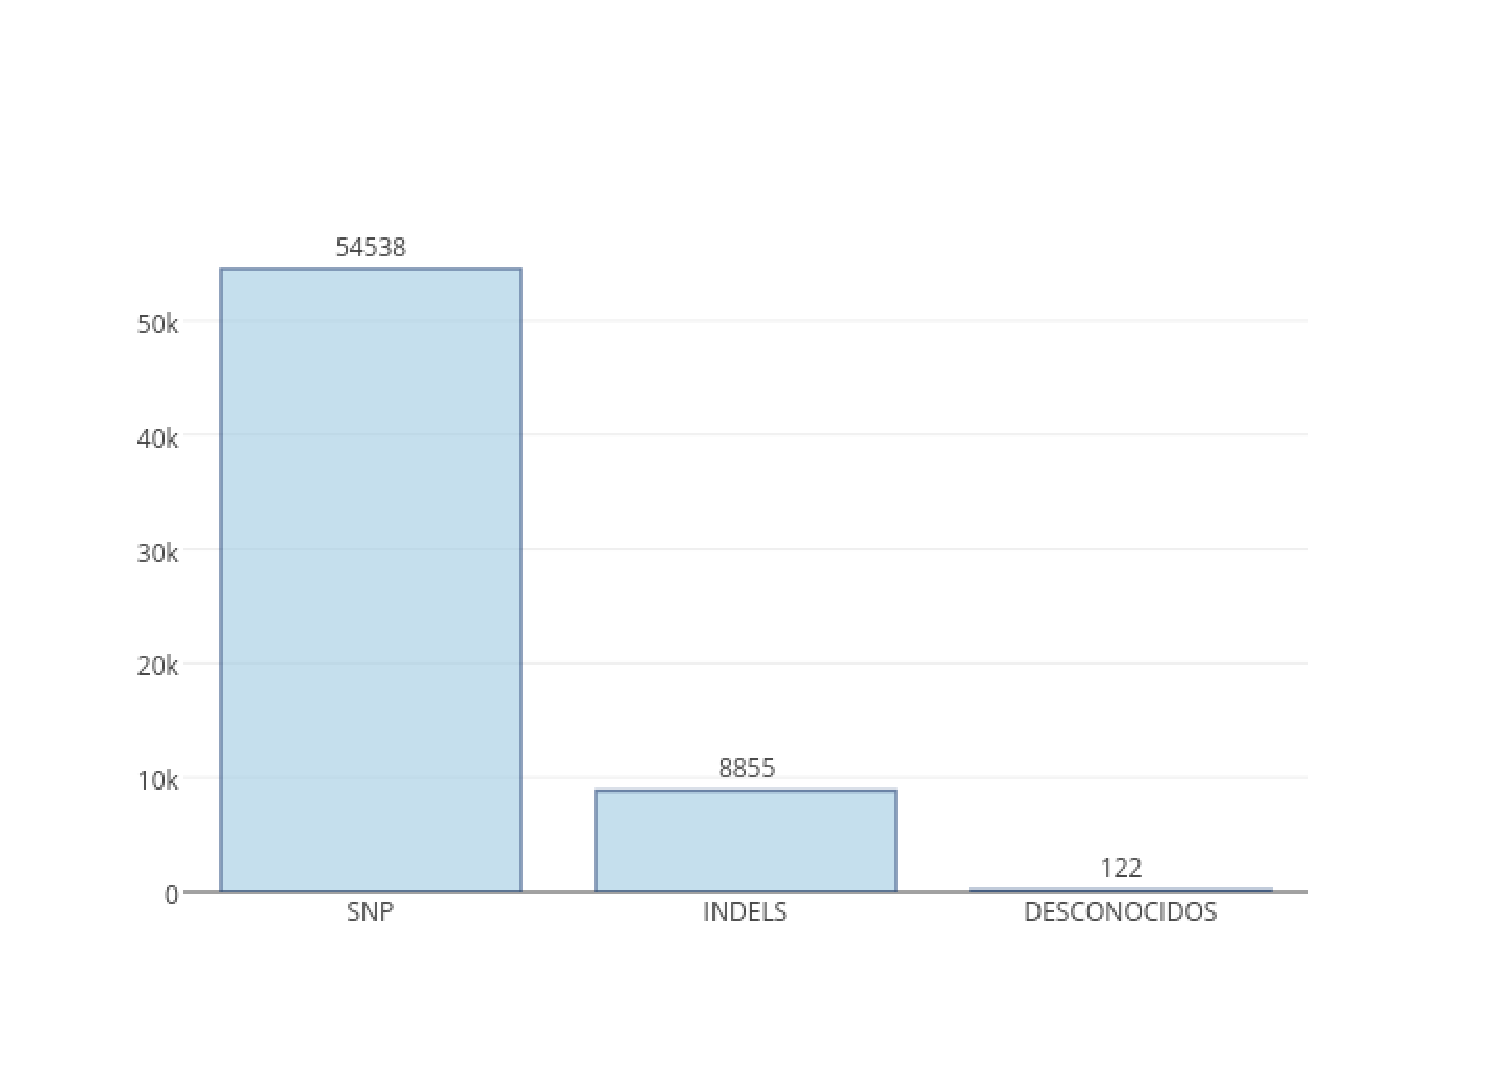
\includegraphics[width=0.5\textwidth]{Kap2/variantesomics}
	\caption{Variantes obtenidas por pipeline} \label{fig:omics}
\end{figure}

Una vez realizado el ``hard filtering" se obtuvo los siguientes resultados: 10425 SNP, 828 Indels y 44 desconocidos, también se tiene las variantes reportadas para el mismo individuo desde la plataforma de illumina con los siguientes resultados: 9601 variantes, 436 indels y 28 desconocidas y representadas en la figura \ref{f:histogramas}.

\begin{figure}[H]
	\subfigure[Variantes obtenidas mediante calibración]{
		\label{f:omics}
		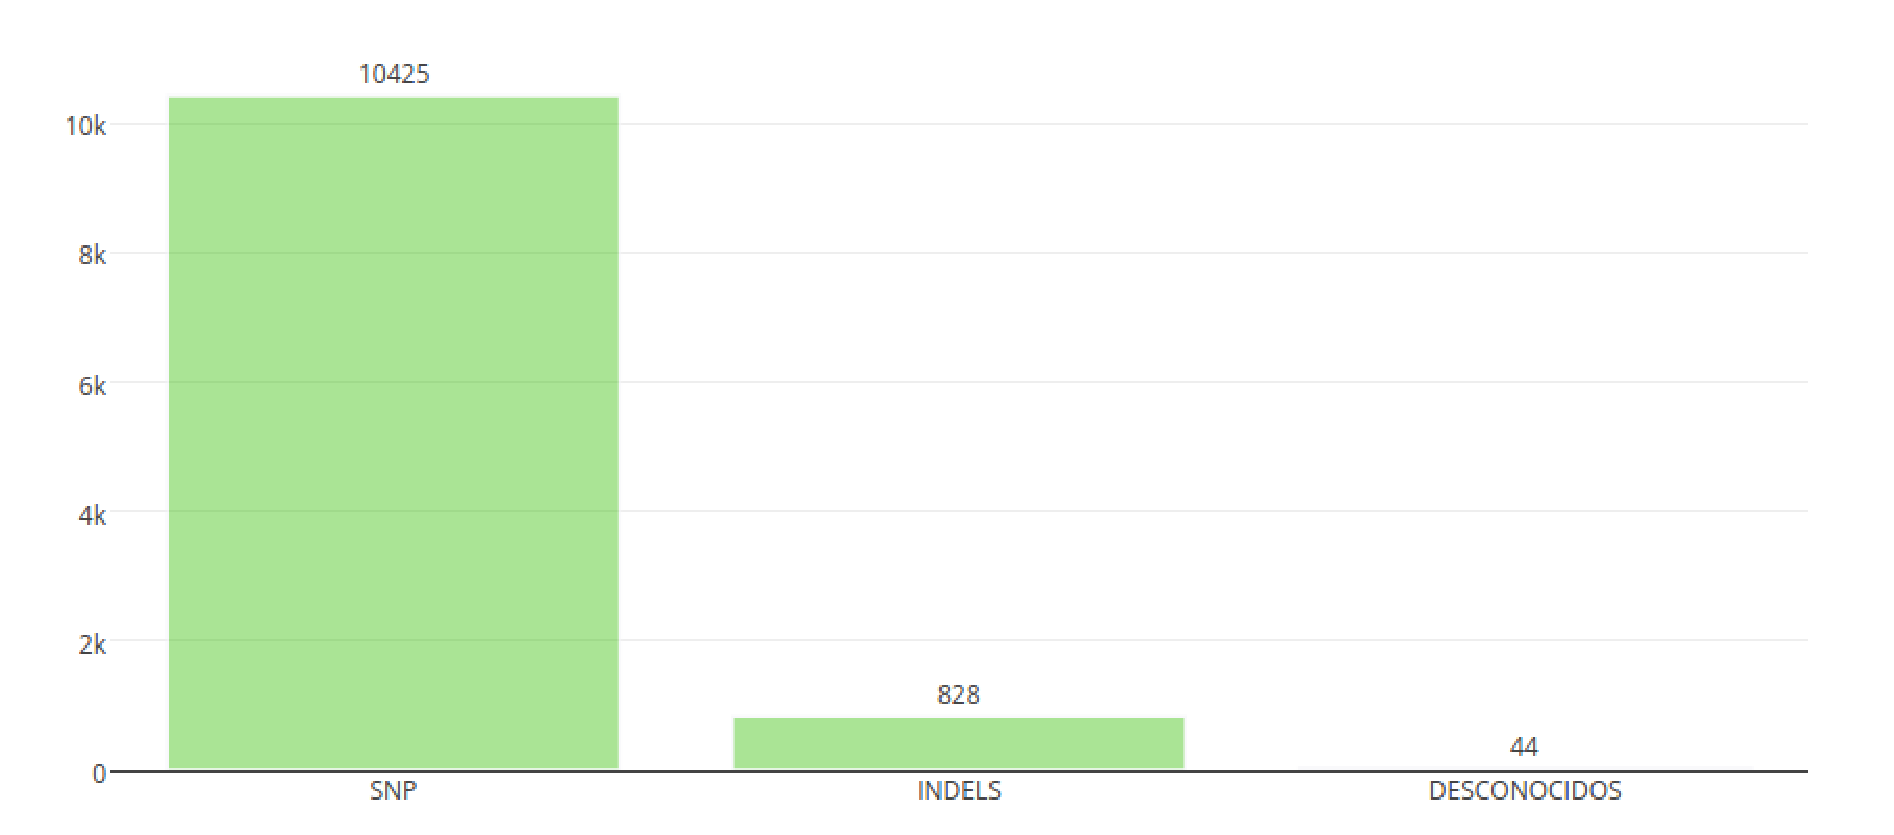
\includegraphics[width=0.5\textwidth]{Kap2/variantescalibradas}}
	\subfigure[Variantes illumina]{
		\label{f:calibradas}
		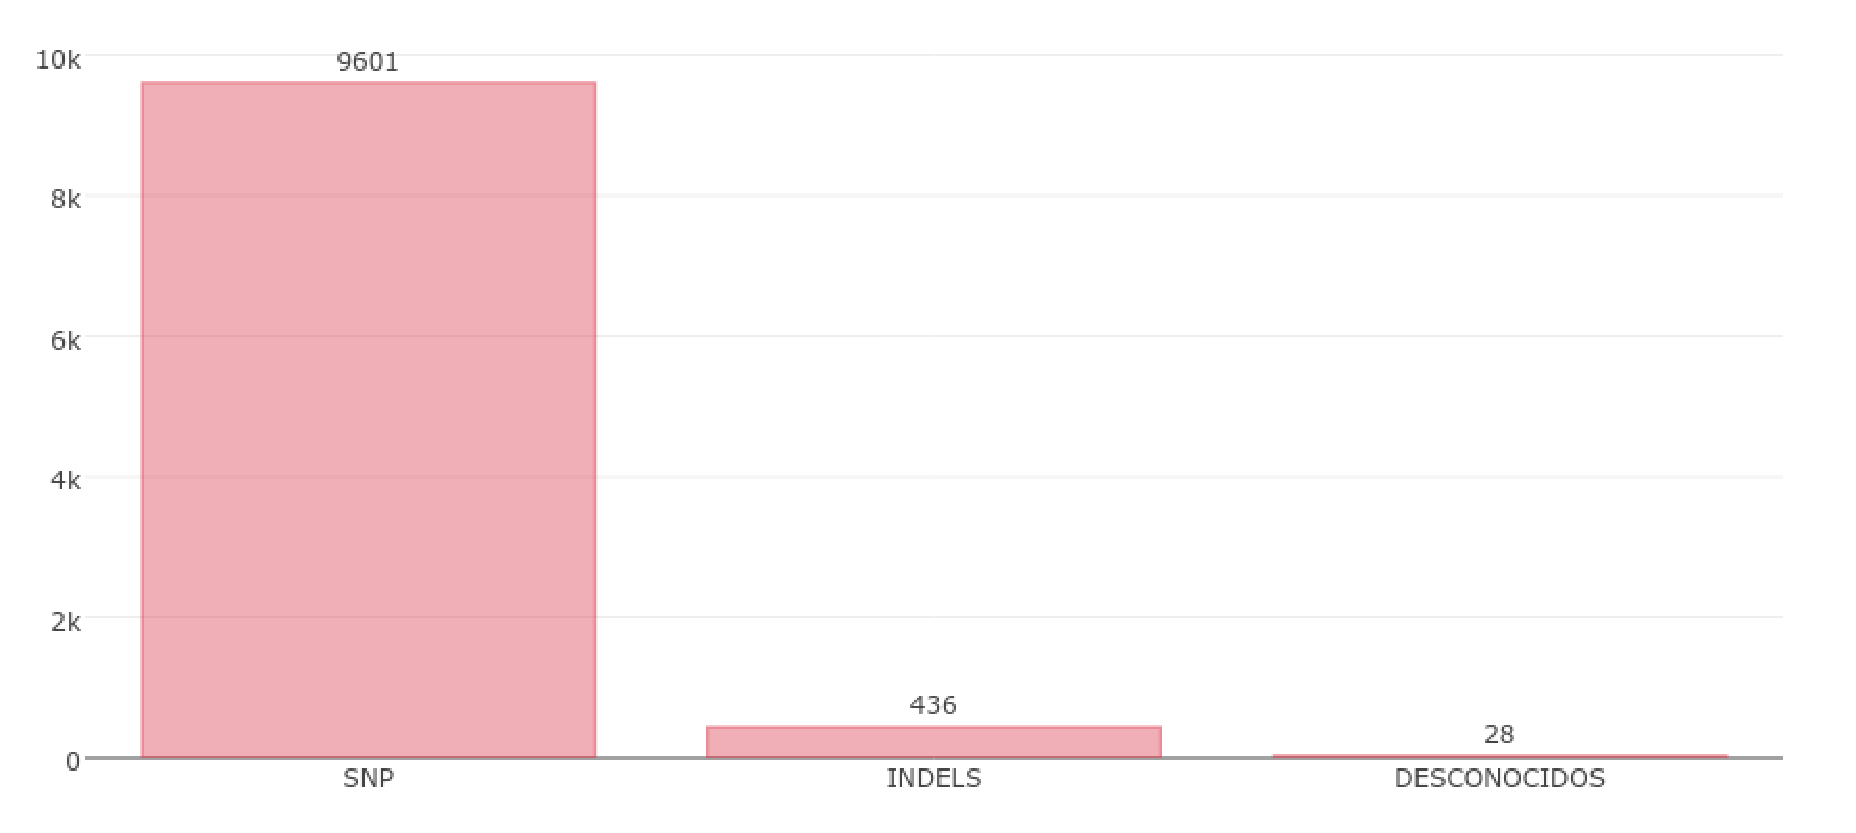
\includegraphics[width=0.5\textwidth]{Kap2/variantesillumina}}
	\caption{Variaciones de la muestra}
	\label{f:histogramas}
\end{figure}

Se realizó una distribución de las variantes según cada técnica sin filtrado (para el caso de omics) para mostrados en las  figuras  \ref{fig:tabla1} y \ref{fig:distribucion}. \\

\begin{figure}[]
	\centering
	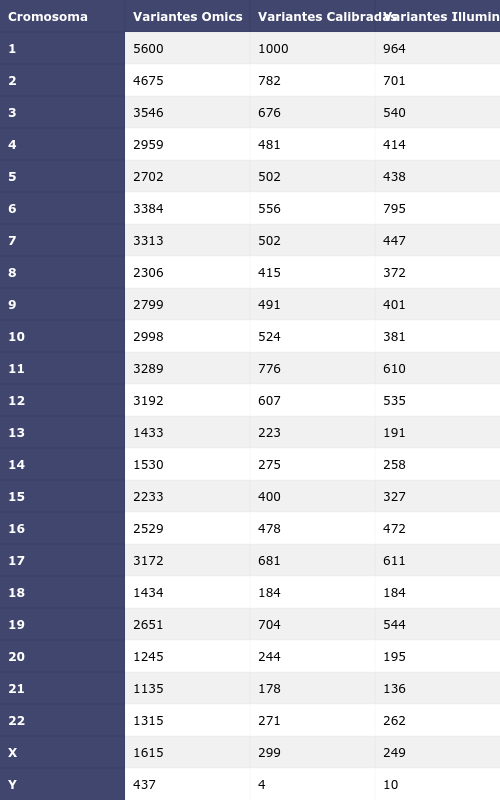
\includegraphics[width=0.4\textwidth]{Kap2/latex_table}
	\caption{Distribución de variantes a lo largo de los cromosomas} \label{fig:tabla1}
\end{figure}

\begin{figure}[]
	\centering
	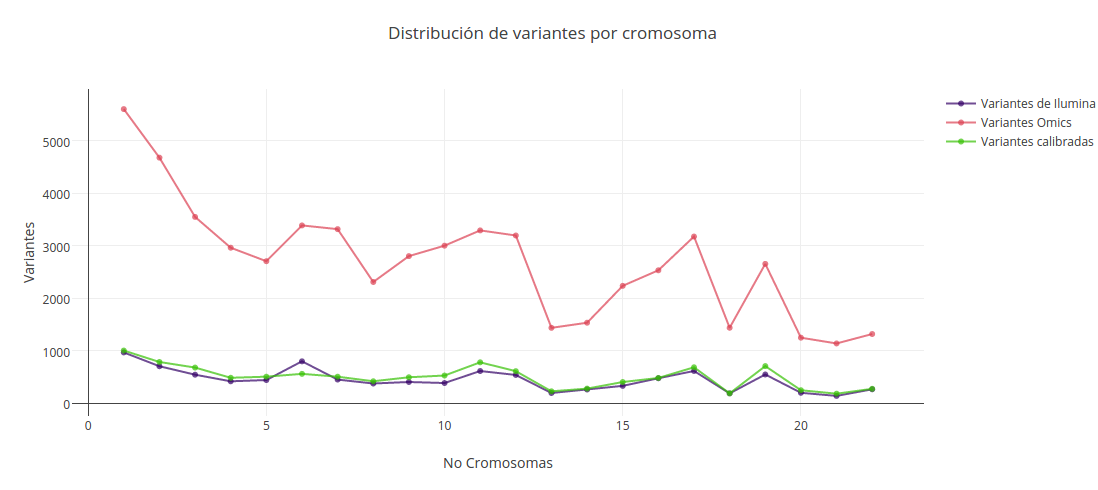
\includegraphics[width=1\textwidth]{Kap2/variaciones}
	\caption{Distribución de variantes a lo largo de los cromosomas.} \label{fig:distribucion}
\end{figure}

Se observa la distribución de las variantes a lo largo del genoma, inicialmente las variantes obtenidas son en grandes cantidades para el modulo de omics, pero conservan el patrón de distribución es similar para los tres casos, incluso cundo se realiza el hard filterin las diferencias en cuanto a la distribución de las variaciones es similar, siendo la mayor para el cromosoma 1 y la menor para el cromosoma Y. \\

Al realizar la comparación entre los dos archivos vcf se obtuvieron los siguientes resultados los archivos vcf de Illumina y los de Omics comparten 49.4 \% d y 44.0 \% de las variantes, y difieren entre un 50.6\% para Illumina y 56-0\% para los datos de omics pipe. Como se refleja la figura \ref{fig:diagrama}. \\

\begin{figure}[]
	\centering
	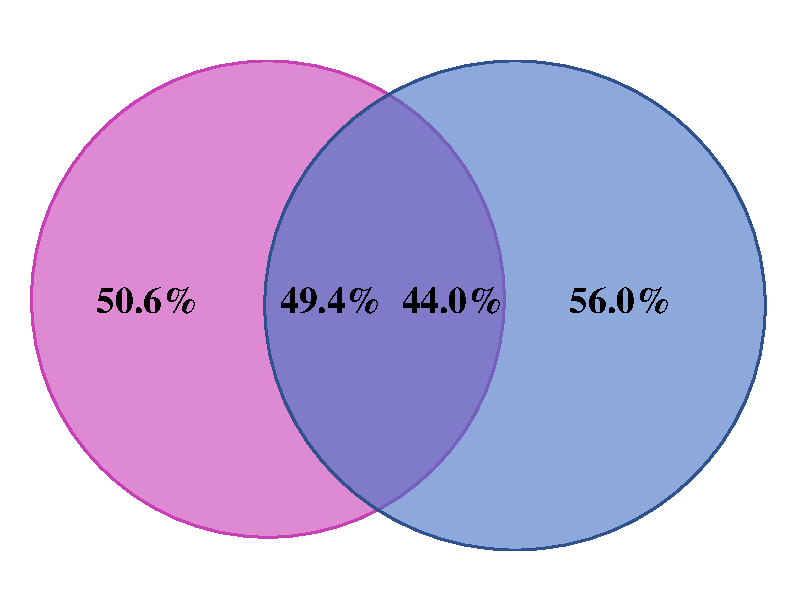
\includegraphics[width=0.3\textwidth]{Kap2/validacion2}
	\caption{Diagrama de relación entre variantes comunes de pipeline y de Illumina} \label{fig:diagrama}
\end{figure}

\subsection*{Variantes de exoma vs variantes de omics}

Una vez obtenidas las regiones se realizó el proceso de ``hard filtering" para el vcf obtenido por el pipe de omics y por el generado por vcftools teniendo los siguientes resultados mostrados por el cuadro \ref{tabla:tabla2}. \\

\begin{table}[H]
	\centering  
	\begin{tabular}{|l|l|l|l|l|}
		\hline
		& \multicolumn{4}{c|}{\textbf{Variantes Exoma}} \\
		\cline{2-5} 
		& SNP  & Indels & Desconocida & Total \\ \cline{2-5}
		\hline 
		\multirow{1}{4cm}{Variantes Omics} & 30893 & 3324 & 0 & 34217 \\ \cline{2-5}
		\hline 
		\multirow{1}{4cm}{Variantes Públicas} & 29749 & 3101 & 0 & 32850 \\ \cline{2-5}
		\hline
	\end{tabular}
	\caption{Variantes obtenidas a partir de un exoma.}
	\label{tabla:tabla2}
\end{table} 

Donde se observa una diferencia de 1367 en el total de las variantes encontradas, para los SNPs se encuentra una diferencia de 1144 y 223 para los indels, no se encuentran variantes que no hayan sido correctamente identificadas. Presentado en los siguientes gráficos \ref{f:histogramas2}. La distribución de las variantes a lo largo de los cromosomas se presenta en la  figura \ref{fig:tabla2}.\\

\begin{figure}[]
	\centering
	\includegraphics[width=0.4\textwidth]{Kap2/latex_table2}
	\caption{Distribución de variantes a lo largo de los cromosomas para los exomas.} \label{fig:tabla2}
\end{figure}

\begin{figure}[H]
	\centering
	\subfigure[Variantes obtenidas por pipeline]{
		\label{f:variantesexo1}
		\includegraphics[width=0.5\textwidth]{Kap2/variantesexo1}}
	\subfigure[Variantes públicas]{
		\label{f:variantesexo2}
		\includegraphics[width=0.35\textwidth]{Kap2/variantesexo2}}
	\caption{Variaciones de la muestras dentro del exoma}
	\label{f:histogramas2}
\end{figure}

La representación gráfica de las variantes sobre la distribución a lo largo de los cromosomas se presenta en la figura \ref{fig:variaciones2}. \\

\begin{figure}[H]
	\centering
	\includegraphics[width=1\textwidth]{Kap2/variaciones2}
	\caption{Distribución de variantes a lo largo de los cromosomas para los exomas} \label{fig:variaciones2}
\end{figure}

En la figura \ref{fig:variaciones2} se observa el comportamiento de la distribución de las variantes para los datos públicos y los datos obtenidos para el pipeline donde se encuentran un comportamiento similar de la distribución, pero se observa que aún hay una mayor cantidad de variantes obtenidas por el pipeline. En la siguiente figura se observa el comportamiento de las variantes públicas con respecto a las variantes del pipeline. \\

\begin{figure}[H]
	\centering
	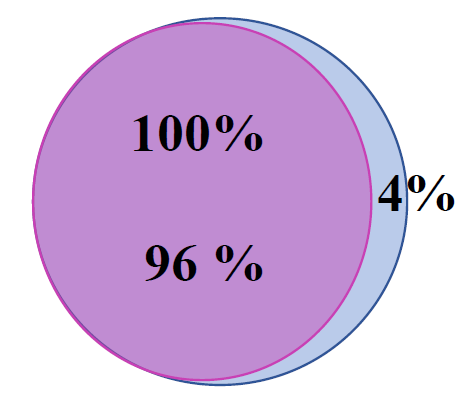
\includegraphics[width=0.2\textwidth]{Kap2/validacion1}
	\caption{Diagrama de relación entre las variantes publicas y las obtenidas por el pipeline.} \label{fig:diagrama2}
\end{figure}

El diagrama de la figura \ref{fig:diagrama2} muestra la comparación entre variantes obtenidas y su respectiva concordancia, donde el 100\% del exoma esta representado en las variaciones encontradas mientras que un 96\% de las variaciones obtenidas por omicspipe corresponden a las variantes del exoma y un 4\% de las variantes no se encontraron dentro del exoma público. \\

GATK realiza un reporte de la evaluación cuando se comparan dos archivos de distintas variaciones, este puede ser abierto como un archivo de texto o cargado directamente en R utilizando la librería \textit{gsalib} que lee el archivo \textit{merged. eval. gatkreport}, esto genera una lista que tiene anidados varios data. frame, dentro de ellos para este caso se tomo el \textit{ValidationReport}. 

El \textit{ValidationReport}  genera una tabla con los verdaderos positivos (\textit{TP}), son las variantes verdaderas definidas como las variantes que previamente han sido identificada en el exoma NA12878, los verdaderos negativos (\textit{TN}), variantes que han sido previamente identificadas pero no son identificadas por el pipeline implementado, los falsos positivos (\textit{FP}) son variantes que no se encuentran en el exoma NA12878, pero que son identificadas por el pipeline y los falsos negativos (\textit{FN}) son las variantes que no están en el exoma NA12878 y que no se identifican, calcula la sensibilidad y la especificidad  y el valor predictivo positivo (PPV). 

\begin{table}[H]
	\begin{center}
		\begin{tabular}{|l|l|}
			\hline 
			\textbf{TP} &  \textbf{FP} \\
			\hline 
			32110 & 1033  \\ \hline
			\textbf{FN} &  \textbf{TN} \\
			\hline
			0 &  0\\ \hline
		\end{tabular}
		\caption{Validación 1. }
		\label{tabla:tabla3}
	\end{center}
\end{table}

El cuadro \ref{tabla:tabla3} refleja que para el conjunto de datos no hay falsos negativos, pero si falsos positivos, es decir  que se obtuvieron 1033 variantes del conjunto de datos que no son reales pero fueron identificadas. (\textit{GATK para calcular estas métricas se compara contra una base de datos que el usuario disponga para determinar variantes existentes}). El cuadro \ref{tabla:tabla4} muestra la sensibilidad, especificidad y el valor predictivo positivo (PPV). 

\begin{table}[h]
	\begin{center}
		\begin{tabular}{|l|l|l|}
			\hline 
			\textbf{Sensibilidad} & \textbf{Especificidad} & \textbf{PPV} \\
			\hline 
			96. 88 & 100 & 100 \\ \hline
		\end{tabular}
		\caption{Validación 2.}
		\label{tabla:tabla4}
	\end{center}
\end{table}

El cuadro \ref{tabla:tabla4} muestra la sensibilidad de 96.88\%, una especificidad del 100\% y un PPV de 100. Además después de realizada la limpieza de los datos se hizo la anotación del archivo vcf obtenido y se filtro para el gen CYP2C19 utilizando la versión gráfica de annovar \cite{Yang2015} y obteniéndose el siguiente resultado: \\

\texttt{chr10, 96541616, 96541616, G, A, exonic, CYP2C19, synonymous SNV, CYP2C19:}

\texttt{NM\_000769:exon5:c. G681A:p. P227P} \\

La representación escrita informa el cromosoma, la posición dentro del genoma y el cambio de posición en el genoma, las siguiente es el cambio Guanina por citocina (representado por sus letras) que es un tipo de variación sinónima, el nombre del gen, su identificador, ubicación exonica y cambio en la posición del exón, finalmente se tiene el cambio en la proteína, la confirmación de que la variante fue encontrada y que es de buena calidad se realizo  con la visualización por medio de la herramienta IGV conectado al clúster como muestra la figura \ref{fig:igv} que muestra el cambio de una G por una A en estado heterocigota. 

\begin{figure}[H]
	\centering
	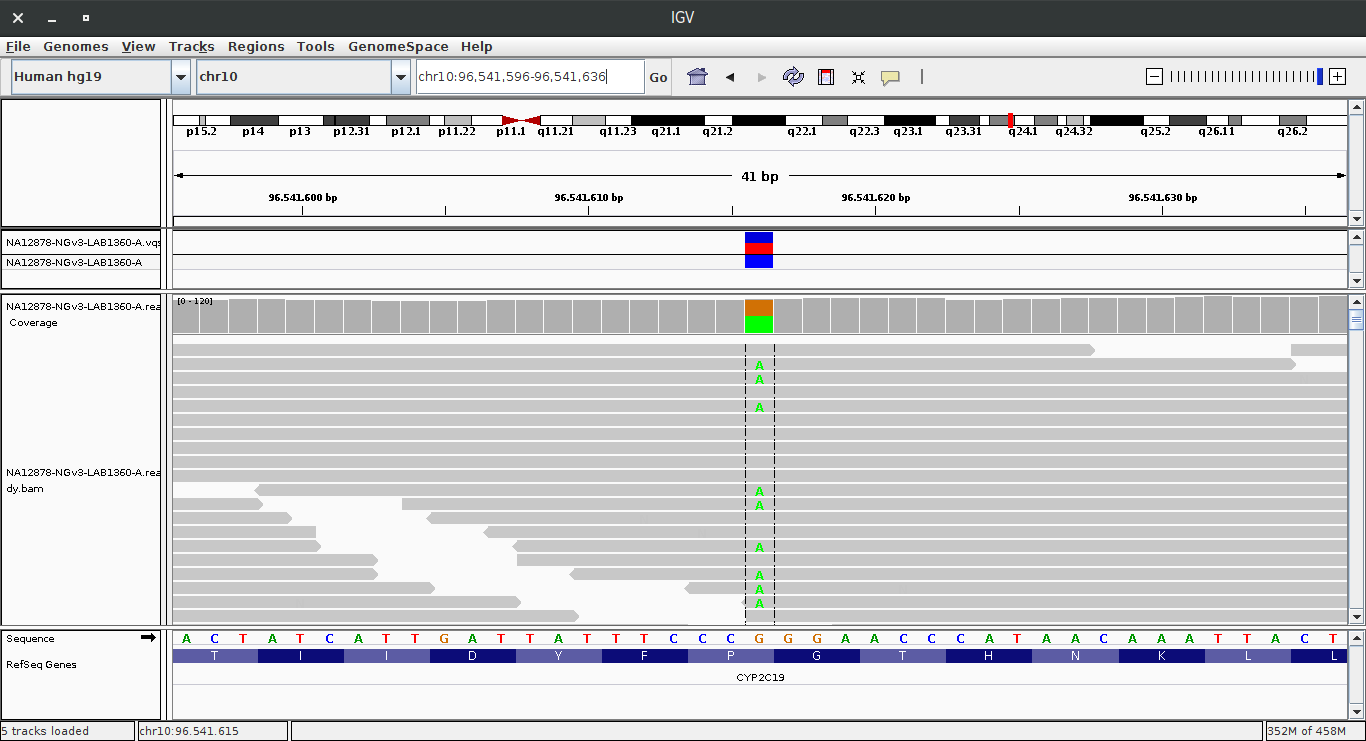
\includegraphics[width=1\textwidth]{Kap2/IGV}
	\caption{Imagen de la variante presente en el exoma público} \label{fig:igv}
\end{figure}

\section{Discusión}

\subsection*{Preprocesamiento}

La revisión de las metricas dadas por el FASTQC report muestran el estado de como están las secuencias antes de ser procesadas, aunque a nivel experimental no dependiendo de las condiciones y el tipo de muestra los niveles de calidad terminan bajando de manera sustancial y depende del analista tomar la decisión de remover secuencias o mantenerlas ya que los diferentes módulos presentan diversas meticas de evaluación de las secuencias \cite{Babraham2016}. \\

El presente conjunto de secuencias FASTQ se encuentra con buenos parámetros de calidad, aunque algunos módulos presentan falla, el percentil, el porcentaje de GC, la distribución del largo de las secuencias, los niveles de duplicación de las secuencias y los valores de K-mer y las secuencias en secuencias cortas de 7 nucleótidos, representan que dentro del conjunto de datos estas secuencias cortas están en la parte inicial de la mayoria de las lecturas obtenidas en la muestra y que posiblemente son secuencias duplicadas que no pertenecen al conjunto de secuencias real, a pesar de que no se encuentran adaptadores, ni representaciones al final de las lecturas. Esto puede llevar a dos caminos, el primero que estas secuencias sean parte de un adaptador (llama la atención que no se encuentren al final de la secuencia)  o que sean errores propios del proceso de secuenciación durante la hibridación de las secuencias y sean representados como duplicaciones de las secuencias originales \cite{Babraham2016}\cite{Pirooznia2014}. \\ 

Además existen otras características que pueden generar impactos negativos dentro del análisis de datos de NGS divididas en dos grupos \cite{Zhou2013}: 

\begin{enumerate}
	\item Lecturas con baja calidad: Las calidades de las lecturas generadas por un secuenciador pueden degradarse durante el proceso de corrido y es común ver fallas al final de la lectura o tener secuencias duplicadas a partir de la amplificación por PCR durante la construcción de las librerías \cite{Zhou2013}. 
	\item Contaminación de las lecturas de especies conocidas o no conocidas en la secuencia objetivo, este error es frecuente y puede se causado por un experimento artificial durante la preparación de la muestra, la construcción de la librería o otro paso experimental, sin embargo las muestras de ADN pueden contener algunos nucleótidos de otras especies, las cuales son difíciles de excluir de manera experimental y por lo tanto si se cree que hay una contaminación, lo ideal es realizar un ``trimming" de las secuencias para remover la contaminación. \textbf{Nota:} Siempre y cuando estén en una baja proporción \cite{Zhou2013}. 
\end{enumerate}

Las secuencias que se  observan pueden ser duplicados de PCR que son un problema crítico cuando los fragmentos están sobre amplificados durante la preparación de las librerías, estos duplicados pueden aumentar a frecuencia alélica e incluir una detección errónea de variantes, esto es muy común los datos de metagenomica, pero en nuestro caso los datos no son datos de metaegenómica si no de un solo individuo llama la atención de que solo estén al inicio de las lecturas y que el final de las lecturas este adecuado esto podría indicar que más que un duplicado de PCR pueda ser un error de secuenciación al inicio de cada nuevo ciclo. \cite{Pandey2016}. \\

Teniendo en cuenta lo anterior se puede inferir que las secuencias duplicadas son bajas y que la calidad de los datos obtenidos son adecuados para continuar con el procesamiento de las secuencias FASTQ, dentro del pipeline se cuenta con una herramienta para remover las secuencias duplicadas (PICARD) y así obtener una calidad optima de los datos. 

\subsection*{Variantes obtenidas}
\subsubsection*{Variantes de illumina y omics pipeline}

En los datos obtenidos para illumina inicialmente reflejados en la tabla \ref{tabla:final}, muestran una alta discordancia ya que inicialmente las variantes no se les aplicó un segundo filtro, siguiendo las recomendaciones de GATK, donde por el pipeline de Omics tiene por defecto el variant quality score racalibration (VQRS) que se basa en machine learning para filtrar las variantes y generar una alta sensibilidad, que es el método más recomendado, pero tiene limitaciones estadísticas y es más robusto que el hard filtering, este es recomendado para datos pequeños \cite{Auwera2014}. \\

Al realizar una calibración de los datos con la calidad y con hard filtering en GATK se obtiene una similitud entre la cantidad de variantes obtenidas por omics pipe con respecto a Illumina, pero aún es posible ver que la distribución de las variantes es similar para ambos conjuntos de datos (véase la figura \ref{fig:distribucion}) y se ve una mayor similitud  después de realizar el filtrado. Esto se presenta debido a que no existe una formula para determinar cuales anotaciones y filtros son adecuados, además el VQSR genera datos de entrenamiento para determinar las variantes. Por esta razón se hacen recomendaciones según lo que se ha observado empíricamente dentro del desarrollo de los algoritmos \cite{Auwera2014}. \\

A pesar de que la distribución de las variante es similar, aun con el filtrado de las variantes existe que la concordancia entre ambas técnicas tiende a ser del 50\% (véase la figura \ref{fig:diagrama}), aunque illumina utiliza GATK la versión implementada es la 1. 6 que en este momento no cuenta con documentación (https://www. broadinstitute. org/gatk/guide/version-history) que illumina utiliza la versión 1. 6 y la función UnifiedGenotyper que presenta algunas inconsistencias para la identificación de indels, mientras que la versión de GATK 3. 5 utiliza la función HaplotyperCaller que mejora el llamado de variantes, y corrige algunas inconsistencias para la identificación de indels \cite{ORawe2013}. Además es la función recomendada para organismos diploides, este se enfoca en dos tipos de identificación inicialmente los SNPs y los indels, y puede identificar cuando hay varios tipos de variantes cercanas a otras \cite{Auwera2014}. \\

Illumina no provee los parámetros utilizados para hacer el llamado de variantes lo que dificulta la comparación entre este pipeline y las variantes reportadas por illumina, además el formato del VCF es el 4. 1 y en la mayoria de las variantes no reporta el valor de la Qual (calidad) para hacer un filtro con el archivo aunque para GATK los valores para el llamado de variantes no son modificados de manera significativa si se realiza un filtro de este tipo \cite{Hwang2015}. Además de que la combinación de BWA con HaplotypeCaller, presentan una mejora con respeto a la identificación de SNPs (BWA-men) y HaplotypeCaller para la identificación de indels \cite{Cornish2015}. 

\subsubsection*{Variantes con un exoma NA12878.}

Para este trabajo se utilizó una muestra del genoma completo de la muestra NA12878 son de 34, 886 variaciones \cite{Cornish2015} en el presente estudio 32850 y el pipeline obtuvo un total de 34217, lo que permite inferir que las variante identificadas son solo de 2036 variaciones (dependiendo de las muestras y los genes que fueron secuenciados) y que se realizó un muestreo partir de un archivo bed. Además si se aplica un filtro para retirar las variaciones con baja calidad, el llamado de variantes de GATK mejora de manera significativa si necesidad de hacer cambios en el preprocesamiento de los datos \cite{Warden2014} \\

Las dos resultados presentan una distribución similar en cuanto a las variantes por cromosoma y no hay variantes desconocidas dentro de la muestra, esto se debe a la alta curación que tiene este exoma, la figura \ref{fig:variaciones2} presenta la distribución a lo largo de los cromosomas donde se presenta leves diferencias entre los datos públicos y los datos generados por el pipeline con una diferencia del 4\% entre las dos resultados, no existen falsos negativos ni verdaderos negativos identificados dentro del conjunto de los datos del pipeline, se presenta una sensibilidad del 96\% que es una buena, dado que las calibraciones y los algoritmos presentan falencias reales para la identificación de variantes \cite{Auwera2014}. Esto se puede corregir por dos vias, aplicando un filtro de Quality by Depth (QD) >= 4 and Fisher Strand Bias (FS) =< 30 para dar un balance  a la sensibilidad y la especificidad \cite{Tsai2016} o aplicando múltiples pipelines. \\


La sensibilidad de un solo pipeline esta en promedio de 95\% al 99\% , que esta dentro del rango de aceptabilidad para la identificación de las variantes \cite{Liu2013}. Para nuestro pipeline tenemos una precisión de 100\%. Lo que nos indica que hay  una baja probabilidad de error. \\

Al realizar la anotación se logro encontrar una de las variantes reportadas para el exoma, en el gen CYP2C19 en la misma posición reportada, con la misma variación mostrando la concordancia entre los resultados del pipeline y la muestra original. \\

Para ambos estudios se presentan archivos intermedios de gran tamaño como son los bam y bai que permiten la visualización de las variantes que pesan entre 6 y 15 gigas para un exoma completo, los datos iniciales pueden pesar entre 1 y 3 gigas (fastq) dependiendo de la cantidad de genes que se hallan secuenciado, lo que requiere de la disponibilidad de un computo para su almacenamiento y procesamiento. 

\section{Conclusiones}

La validación de un pipeline para la identificación de variantes requiere la utilización de herramientas computacionales de HPC para hacerse de manera eficiente. Es necesario que se tengan conocimientos de programación básica y biología molecular, con el fin de definir los parámetros óptimos para la implementación un pipeline. \\ 

La cantidad de herramientas y parámetros para aplicar son diversos y dependen del investigador decidir cuales son los mejores y que filtros van a ser utilizados, dado que a pesar de la existencia de protocolos no hay un consenso de cual o cuales son los mejores y estos dependen del conjunto de datos obtenido. \\ 

El llamado de variantes es bueno para el presente estudio, pero hay la posibilidad de mejorar la implementación de los parámetros de filtrado y el proceso de anotación (implicación del cambio de las variantes), además generar un pipeline alternativo para la verificación de las variantes que están siendo identificadas y poder aumentar la sensibilidad. \\

Es necesario crear o generar la manera de optimizar los tiempos de ejecución de las tareas de una manera más eficiente a la dada por el omics-pipe. 

\section*{Resumen}

Se realizó la implementación y validación de un pipeline para la identificación variantes a partir de secuencias de exomicas a partir de muestras de pacientes colombianos y del genoma público de la muestra NA12878 donde se identificaron las variantes que están presentes en el mismo, teniendo en cuenta las buenas practicas para el llamado de variantes lo que permitió desarrollar un mecanismo para obtener variantes de buena calidad. 